\subsection{Datamodel}
Het Datamodel bestaat uit 4 \textbf{objecten} wat in zijn geheel leid naar de uitendelijke data die naar de frontend wordt gestuurd.
Deze objecten zijn Item Definition, Item Value, Visual Component en ItemVisual.

\whitespace[2]
\textbf{Item Value}: De Item Value slaat encapsuleert de content/data van het systeem op.
Item Values kunnen meerdere Item values bevatten, waardoor je een geneste structuur krijgt.
De Item value bevat ook 1 of meerdere FieldValueEntityBase.
Deze abstracte class zorgt er voor dat er verschillende data types kunnen opgeslagen worden in het het zelfde item.
In het klassen diagram (zie figuur \ref{fig:ItemValueEntityClassDiagram}) zijn de huidige implementatie mogelijkheden.
Deze zijn String,Bool,Int en Api deze lijst zou in de toekomst uitgebruikt kunnen worden.
Een bezondere is de Api FieldType, met dit veld maakt je een http get request naar een ander url.
Hierdoor kan je dynamisch externe content ophalen, bijvoorbeelde de Oembed data van een youtube video.

\whitespace[2]
\begin{graphic}
    \captionsetup{type=figure}
    \caption{klassen diagram ItemValue}
    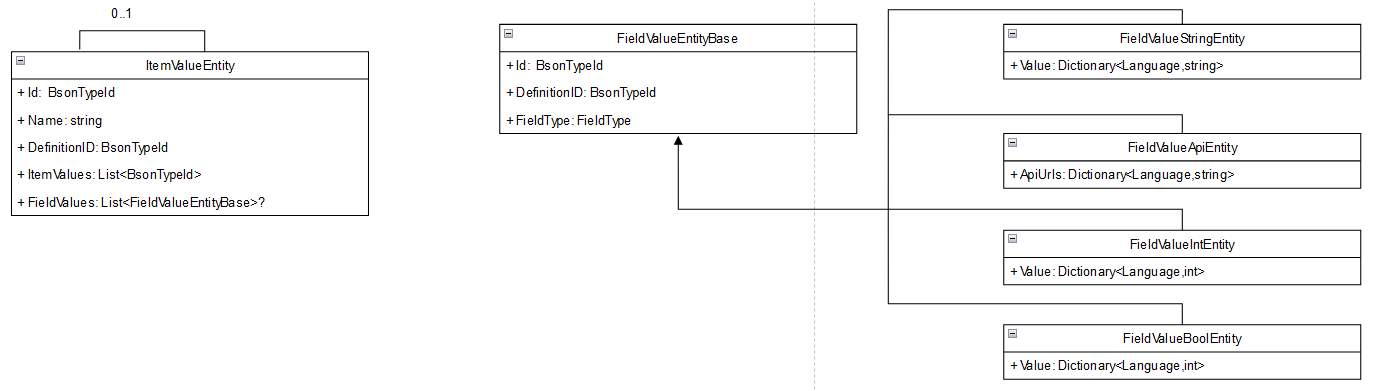
\includegraphics[scale=0.7]{ItemValueEntityClassDiagram.png}
    \label{fig:ItemValueEntityClassDiagram}
\end{graphic}

\whitespace[2]
\textbf{Item Definition}: Om structuur te geven aan de Item values wordt er gebruik gemaakt van een item Definition.
        De belangrijkste functionaliteit van de definition is om aan te geven welke velden er op verschillende items zitten en welke daarvan verplicht zijn.

\whitespace[2]
\begin{graphic}
    \captionsetup{type=figure}
    \caption{klassen diagram ItemDefinition}
    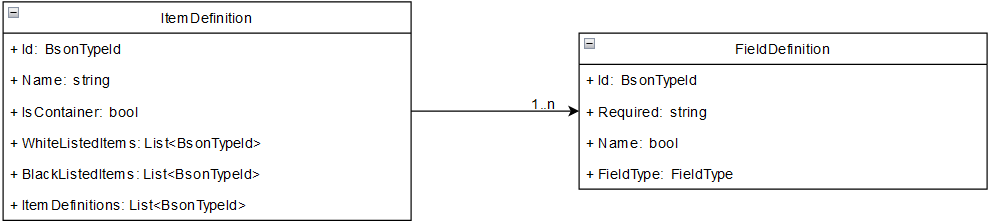
\includegraphics[scale=0.8]{ItemDefinitionClassDiagram.png}
    \label{fig:ItemDefinitionClassDiagram}
\end{graphic}

\whitespace[2]
\textbf{VisualComponent}: Om de data te renderen moeten er components gebruikt worden in de frontend om dit af te handelen waar nodig.
De VisualComponent wordt gebruikt om deze componenten aan te geven welke er zijn en welke definition er bij hoordt.

\whitespace[2]
\begin{graphic}
    \captionsetup{type=figure}
    \caption{Klassen diagram VisualComponent}
    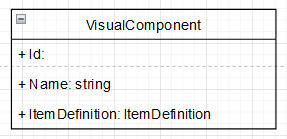
\includegraphics[scale=0.8]{VisualComponentEntityClassDiagram.png}
    \label{fig:VisualComponentEntityClassDiagram}
\end{graphic}

\whitespace[2]
\textbf{ItemVisual}: Dit is het object dat de VisualComponent en de Item Value samen voegt tot een geheel waardoor er content gerenderd kan worden op de pagina.
Verder geeft dit object ook aan welke mogelijke stijling of layout op het item moet worden toegepast.

\whitespace[2]
\begin{graphic}
	\captionsetup{type=figure}
	\caption{Klassen diagram ItemVisual}
	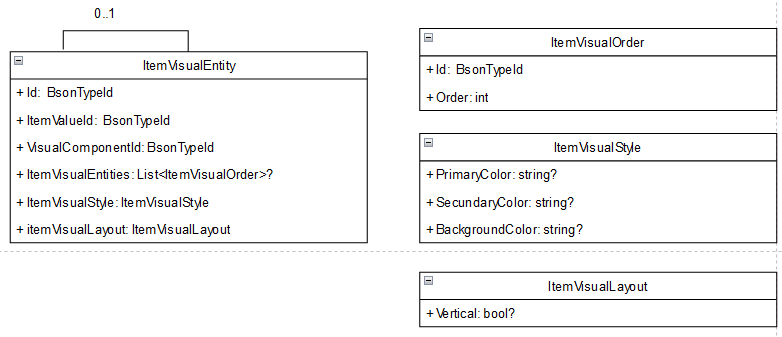
\includegraphics[scale=0.8]{ItemVisualEntityClassDiagram.png}
	\label{fig:ItemVisualEntityClassDiagram}
\end{graphic}

\whitespace[2]
Om de data te renderen op een froentend wordt er gebruik van de ItemVisualDTO zie figuur \ref{fig:ItemVisualDTOClassDiagram}.
De data wordt hier genest en geordend op basis van de ordering.

\whitespace[2]
\begin{graphic}
	\captionsetup{type=figure}
	\caption{Klassen diagram ItemVisual}
	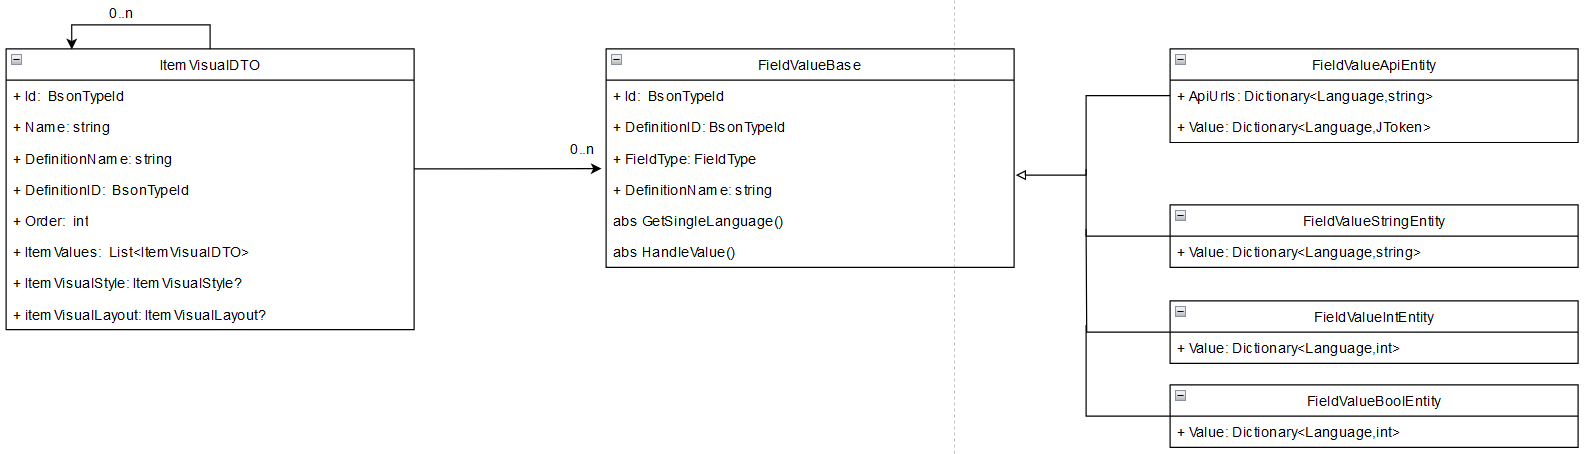
\includegraphics[scale=0.7]{ItemVisualDTO.png}
	\label{fig:ItemVisualDTOClassDiagram}
\end{graphic}
